\let\negmedspace\undefined
\let\negthickspace\undefined
\documentclass[journal]{IEEEtran}
\usepackage[a5paper, margin=10mm, onecolumn]{geometry}
%\usepackage{lmodern} % Ensure lmodern is loaded for pdflatex
\usepackage{tfrupee} % Include tfrupee package

\setlength{\headheight}{1cm} % Set the height of the header box
\setlength{\headsep}{0mm}     % Set the distance between the header box and the top of the text

\usepackage{gvv-book}
\usepackage{gvv}
\usepackage{cite}
\usepackage{amsmath,amssymb,amsfonts,amsthm}
\usepackage{algorithmic}
\usepackage{graphicx}
\usepackage{textcomp}
\usepackage{xcolor}
\usepackage{txfonts}
\usepackage{listings}
\usepackage{enumitem}
\usepackage{mathtools}
\usepackage{gensymb}
\usepackage{comment}
\usepackage[breaklinks=true]{hyperref}
\usepackage{tkz-euclide} 
\usepackage{listings}
% \usepackage{gvv}                                        
\def\inputGnumericTable{}                                 
\usepackage[latin1]{inputenc}                                
\usepackage{color}                                            
\usepackage{array}                                            
\usepackage{longtable}                                       
\usepackage{calc}                                             
\usepackage{multirow}                                         
\usepackage{hhline}                                           
\usepackage{ifthen}                                           
\usepackage{lscape}
\begin{document}

\bibliographystyle{IEEEtran}
\vspace{3cm}

\title{CHAPTER - 9\\Differential Equations}
\author{EE24BTECH11061 - Rohith Sai}
% \maketitle
% \newpage
% \bigskip
{\let\newpage\relax\maketitle}

\renewcommand{\thefigure}{\theenumi}
\renewcommand{\thetable}{\theenumi}
\setlength{\intextsep}{10pt} % Space between text and floats

\numberwithin{figure}{enumi}
\renewcommand{\thetable}{\theenumi}

\section*{Exercise : 9.7 (Miscellaneous)}
\begin{enumerate}
\item [10)] Solve the differential equation  $y e^{\frac{x}{y}} \, dx = \left(x e^{\frac{x}{y}} + y^2\right) \, dy $

\textbf{Solution (using the Method of Finite Differences):}\\
The given differential equation can be rearranged as:
\begin{align}
     y e^{\frac{x}{y}} \, dx = \left(x e^{\frac{x}{y}} + y^2\right) \, dy
\end{align}

Let's express it in the form of \( \frac{dx}{dy} \):
\begin{align}
    \frac{dx}{dy} &= \frac{x}{y} + y e^{-\frac{x}{y}}
\end{align}

We will solve this using Euler's method, which approximates the solution iteratively. Using the finite difference approximation:
\begin{align}
    x_{n+1} &= x_n + h \cdot \left(\frac{x_n}{y_n} + y_n e^{-\frac{x_n}{y_n}}\right)
\end{align}

Let $y_0$ be the initial $y$-value, $x_0$ be the initial $x$-value. Let the step size $h$ be 0.001. The first few iterations are:
\begin{align*}
    y_1 &= y_0 + h, & x_1 &= x_0 + h \cdot \left(\frac{x_0}{y_0} + y_0 e^{-\frac{x_0}{y_0}}\right) \\
    y_2 &= y_1 + h, & x_2 &= x_1 + h \cdot \left(\frac{x_1}{y_1} + y_1 e^{-\frac{x_1}{y_1}}\right) \\
    &\vdots  & \vdots \\
    y_n &= y_{n-1} + h, & x_n &= x_{n-1} + h \cdot \left(\frac{x_{n-1}}{y_{n-1}} + y_{n-1} e^{-\frac{x_{n-1}}{y_{n-1}}}\right)
\end{align*}

\textbf{Solution (using the General Method):}\\
The given differential equation is:
\begin{align}
    y e^{\frac{x}{y}} \, dx &= \left(x e^{\frac{x}{y}} + y^2\right) \, dy
\end{align}

Dividing both sides by \( y e^{\frac{x}{y}} \), we get:
\begin{align}
    dx &= \frac{x + y^2 e^{-\frac{x}{y}}}{y} \, dy
\end{align}

Rearranging to express \( \frac{dx}{dy} \):
\begin{align}
    \frac{dx}{dy} &= \frac{x}{y} + y e^{-\frac{x}{y}}
\end{align}

Using the substitution \( v = \frac{x}{y} \), we have:
\begin{align}
    x &= vy \quad \text{and} \quad \frac{dx}{dy} = v + y \frac{dv}{dy}
\end{align}

Substituting these into the equation and simplifying:
\begin{align}
    v + y \frac{dv}{dy} &= v + y e^{-v}
\end{align}

Dividing by \( y \), we get:
\begin{align}
    \frac{dv}{dy} &= e^{-v}
\end{align}

Integrating both sides:
\begin{align}
    \int e^v \, dv &= \int 1 \, dy \\
    \implies e^v &= y + C
\end{align}

Substituting back \( v = \frac{x}{y} \):
\begin{align}
    e^{\frac{x}{y}} &= y + C
\end{align}

Taking the logarithm of both sides:
\begin{align}
    \frac{x}{y} &= \ln(y + C)
\end{align}

Multiplying by \( y \):
\begin{align}
    x &= y \ln(y + C)
\end{align}
Let's assume $C = 0$ and $y=1$. On substituting these values in equation (14), we get $x = 0$.\\
Therefore, the equation is
\begin{align*}
    x = y \ln{\brak{y}}
\end{align*}
Therefore, the curve generated using both the above mentioned methods for the given differential equation (1) is shown below:
\begin{figure}[H]
    \centering
    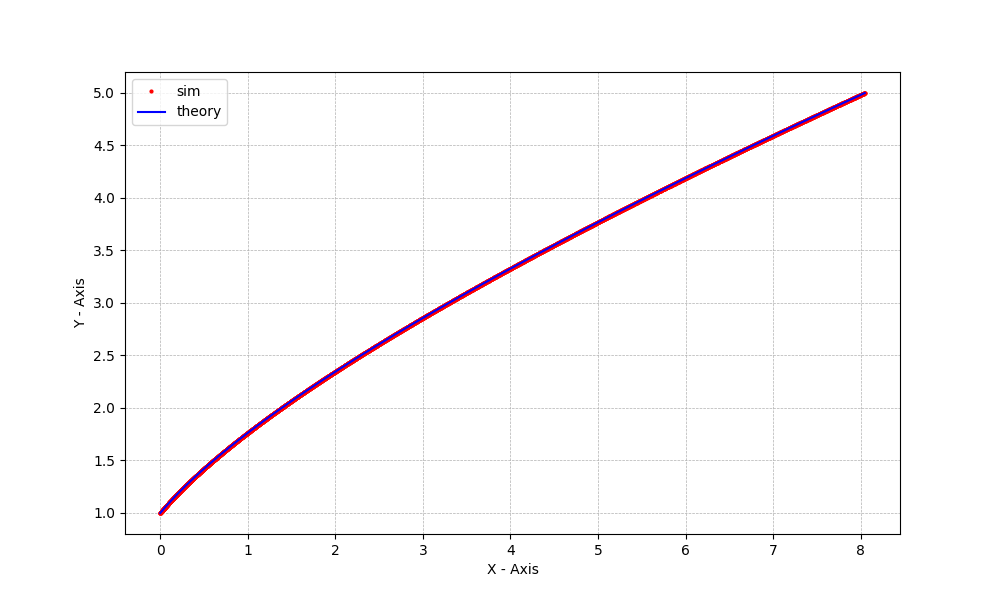
\includegraphics[width = \columnwidth]{figs/fig.png}
\end{figure}
\end{enumerate}
\end{document}